\documentclass{article}

\usepackage{graphicx}
\usepackage{tikz}
\usepackage{tikzsymbols}
\usetikzlibrary{calc,patterns,shapes.geometric}
\pagestyle{empty}
\usepackage[margin=0pt]{geometry}
\geometry{papersize={14in,12in}}

\def\centerarc[#1](#2)(#3:#4:#5){\draw[#1] ($(#2)+({#5*cos(#3)},{#5*sin(#3)})$) arc (#3:#4:#5);}

\begin{document}
	\begin{figure}
		\centering
		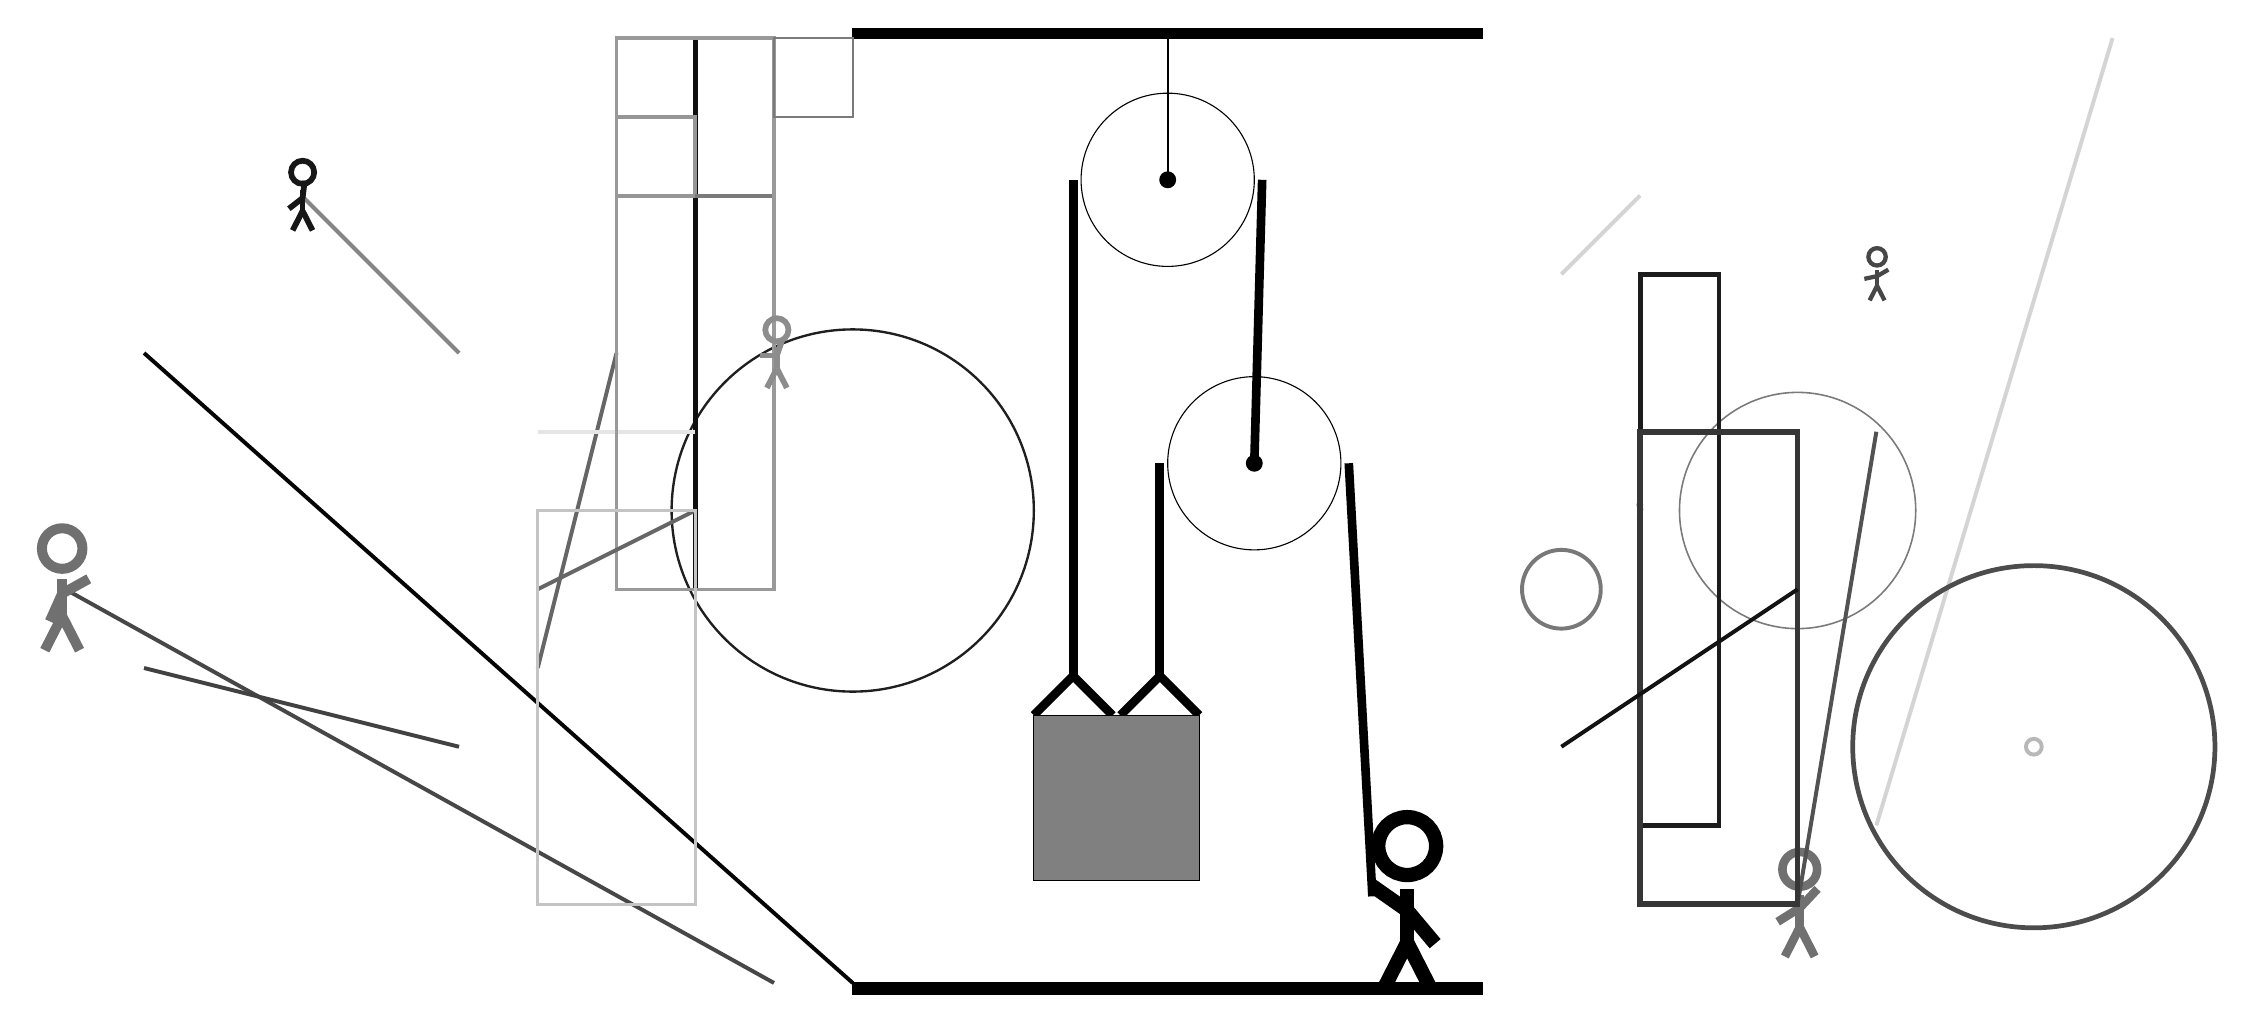
\begin{tikzpicture}
			%%%%% START %%%%%
			
			\draw[fill=black] (-2, 9) rectangle (6, 9.125);
			
			\draw (2, 7.2) circle (1.1);
			\draw[fill=black] (2, 7.2) circle (0.1);
			\draw[thick] (2, 7.2) -- (2, 9);
			
			\draw [line width=0.2mm, color=black!52](10, 3) circle (1.5);
			
			\draw[line width=0.5mm, color=black!98](-2, -3) -- (-11, 5);
			\draw[line width=0.5mm, color=black!60](-6, 1) -- (-5, 5);
			\node[line width=0.7mm, color=black!25] at (8, 3) {\Strichmaxerl[1][86][31]};
			\draw [line width=0.3mm, color=black!88](-2, 3) circle (2.3);
			\draw[line width=0.6mm, color=black!94] (-4, 9) rectangle (-4, 2);
			
			\node[line width=0.3mm, color=black!56] at (10, -2) {\Strichmaxerl[6][32][47]};
			\draw[line width=0.5mm, color=black!17](11, -1) -- (14, 9);
			\draw[line width=0.5mm, color=black!72](-3, -3) -- (-12, 2);
			\draw [line width=0.5mm, color=black!28](13, 0) circle (0.1);
			\draw[line width=0.5mm, color=black!68](10, -2) -- (11, 4);
			\draw[line width=0.5mm, color=black!41] (-4, 7) rectangle (-5, 8);
			\draw[line width=0.5mm, color=black!52](-3, 7) -- (-4, 7);
			
			\draw[line width=0.6mm, color=black!89] (8, -1) rectangle (9, 6);
			\draw[line width=0.5mm, color=black!10](-4, 4) -- (-6, 4);
			\draw[line width=0.4mm, color=black!40] (-3, 2) rectangle (-5, 9);
			
			\draw [line width=0.5mm, color=black!53](7, 2) circle (0.5);
			
			\draw[line width=0.3mm, color=black!52] (-2, 9) rectangle (-3, 8);
			\draw[line width=0.7mm, color=black!79] (8, -2) rectangle (10, 4);
			\node[line width=0.5mm, color=black!45] at (-3, 5) {\Strichmaxerl[4][0][71]};
			\node[line width=0.7mm, color=black!56] at (-12, 2) {\Strichmaxerl[7][66][29]};
			\draw [line width=0.6mm, color=black!70](13, 0) circle (2.3);
			\draw[line width=0.5mm, color=black!48](-7, 5) -- (-9, 7);
			\draw[line width=0.5mm, color=black!93](7, 0) -- (10, 2);
			\node[line width=0.2mm, color=black!72] at (11, 6) {\Strichmaxerl[3][12][30]};
			
			\draw[line width=0.5mm, color=black!60](-4, 3) -- (-6, 2);
			\draw[line width=0.5mm, color=black!74](-7, 0) -- (-11, 1);
			\draw[line width=0.4mm, color=black!23] (-4, 3) rectangle (-6, -2);
			\draw[line width=0.5mm, color=black!17](8, 7) -- (7, 6);
			
			\node[line width=0.4mm, color=black!91] at (-9, 7) {\Strichmaxerl[4][38][83]};
			
			\draw (3.1, 3.6) circle (1.1);
			\draw[fill=black] (3.1, 3.6) circle (0.1);
			
			\draw[line width = 1.1mm]  (0.3, 0.4) -- (0.8, 0.9) -- (1.3, 0.4);
			\draw[line width = 1.1mm]  (1.4, 0.4) -- (1.9, 0.9) -- (2.4, 0.4);
			\draw[fill=black!50] (0.3, 0.4) rectangle (2.4, -1.7);
			
			\draw[line width = 1.1mm] (0.8, 7.2) -- (0.8, 0.9);
			\centerarc[line width = 1.1mm](2, 7.2)(0:180:1.2000000000000002);
			\draw[line width = 1.1mm] (3.2, 7.2) -- (3.1, 3.6);
			\draw[line width = 1.1mm] (1.9, 3.6) -- (1.9, 0.9);
			\centerarc[line width = 1.1mm](3.1, 3.6)(0:180:1.2000000000000002);
			\draw[line width = 1.1mm] (4.3, 3.6) -- (4.6, -1.9);
			
			\node at (5, -2) {\Strichmaxerl[10][-35][-50]};
			
			\draw[fill=black] (-2, -3) rectangle (6, -3.15);
			
			%%%%% END %%%%%
		\end{tikzpicture}
	\end{figure}	
\end{document}